\documentclass[12pt,oneside,a4paper]{article}
% Umlaute direkt nutzen (Text muss direkt in utf8 vorliegen => Default bei sublime): statt
% \"A, \"O, \"U, \"a, \"o, \"u und \ss{} direkt Ä, Ö, Ü, ä, ö, ü und ß im Text engeben
\usepackage[utf8]{inputenc}  % Umlaute direkt eingeben (ggf. latin1 statt utf8)
\usepackage[T1]{fontenc}     % Ausgabe der Umlaute
\usepackage{lmodern}

\usepackage[dvips]{graphicx}       % alles zum Grafiken einbinden
\graphicspath{ {./images/} }       % pointer to subdir for all images

\usepackage{caption}
\usepackage{subcaption}

\usepackage{eurosym}               % Eurosymbol

\usepackage[centertags]{amsmath}   % Mathekram: amstex
\usepackage{amssymb}
\usepackage{cases}
\usepackage{latexsym}              % math symbols
\usepackage{exscale}               % Summen-/Integralzeichen in richtiger Groesse

\usepackage[dvipsnames]{xcolor}    % Textcolor for dvips w/ standard color names
\usepackage{fancyhdr}              % to change header and footers

% Deutsch als Hauptsprache im Dokument (Layout von Datum, Trennungsregeln etc.)
% Umschaltbar mit \selectlanguage{}
\usepackage[main=english,ngerman]{babel}  % support "Neue Rechtschreibung"

\usepackage[version=4]{mhchem}     % Chemische Formeln (muss nach amsmath kommen!)

\usepackage{hyperref}  % must be imported as last package!
\hypersetup{
    colorlinks=true,
    linkcolor=blue,
    filecolor=magenta,      
    urlcolor=cyan,
    pdftitle={Overleaf Example},
    pdfpagemode=FullScreen,
    }

% \DeclareMathSizes{11}{19}{13}{9} \DeclareMathSizes{12}{20}{14}{10}  % Larger formulas
% vs. text

\title{Neural Network Basics}
\author{Daniel Hug}
\date{August and September 2023}


\pagestyle{fancy}       % Turn on the style
\fancyfoot{}            % Clear the footer
\fancyfoot[R]{\thepage} % Set the right side of the footer to be the page numberå

% new commands for partial derivatives
\newcommand{\pd}[2]{\ensuremath{\frac{\partial {#1}}{\partial {#2}}}}


\begin{document}

\maketitle

% no paragraph indentation on first line
\setlength{\parindent}{0pt}

\section{Neural Net Basics}

Sources:
\begin{itemize}
    \item \url{http://neuralnetworksanddeeplearning.com}
    \item \url{https://brilliant.org/wiki/feedforward-neural-networks/\#formal-definition}
    \item \url{https://brilliant.org/wiki/backpropagation/}
\end{itemize}


\newpage

\subsection{Neural Net Definitions}

In this document we look into a neural network based on perceptron cells with an
activation function. A single perception can be regarded as a linear classifier, i.e. it
is able to output which of two linearly separable data sets a point belongs to. In order
to classify more complex data sets, layers of perceptrons are required.

\begin{figure}[h] \centering
    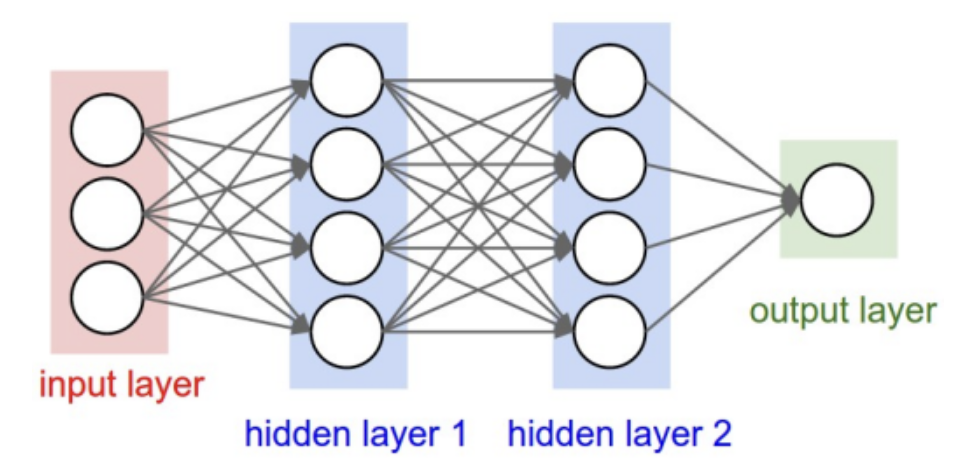
\includegraphics[width=0.75\textwidth]{neural_network} \caption{A fully
    connected multi-layer neural network with three inputs, two
    hidden layers, each with four perceptron nodes and an output layer with a
    single output node. (Source: https://towardsdatascience.com)} \label{fig:neural_network}
\end{figure}

A neural net consists of $L$ layers with $n^l$ nodes in each layer $l=[0,L)$. For the
input layer $(l=0)$ the nodes are simple input nodes, while for the remaining layers
consist of perceptron nodes (see figure~\ref{fig:percptron}). \\

A perceptron with an arbitrary activation function looks like this:
\begin{figure}[h] \centering 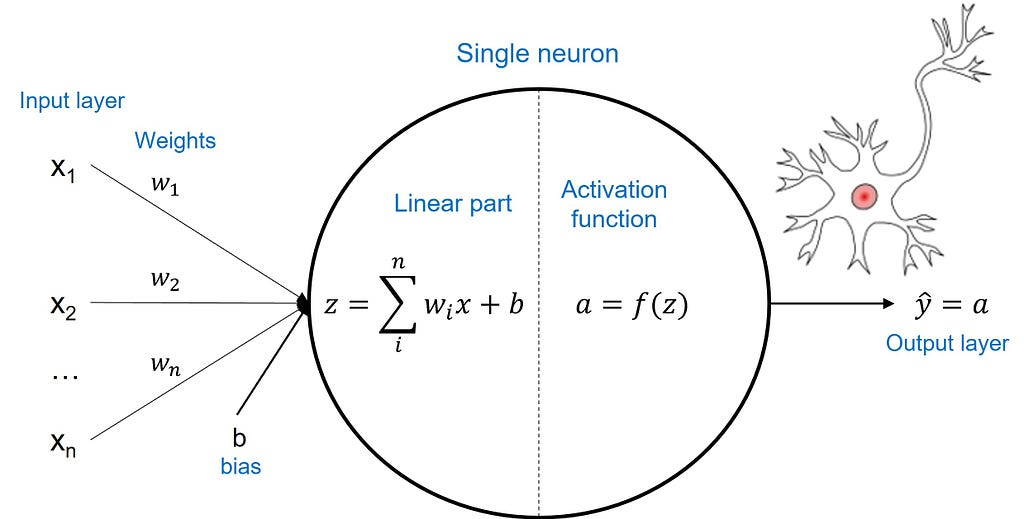
\includegraphics[width=0.75\textwidth]{single_neuron}
    \caption{A node of a neural network with inputs, bias and activiation function.
    (Source: https://towardsai.net)}
    \label{fig:percptron}
\end{figure}

Definitions:
\begin{enumerate}
    \item The training dataset $X$ consisting of input-output pairs $(\vec{x}_i,
    \vec{y}_i)$, where $\vec{x}_i$ is the input and $\vec{y}_i$ is the desired or target
    output of the network on the input $\vec{x}_i$. The set of input-output training pairs
    of size $N$ is denoted $X = \{(\vec{x}_1,\vec{y}_1), \dots, (\vec{x}_N,\vec{y}_N)\}$.

    \item A feedforward neural network has (learning) parameters, i.e.\ weights and
    biases, that are collectivly denoted $\theta$. The nodes in different layers are fully
    connected, while there are no connections between nodes in the same layer. For
    backpropagation the parameters of primary interest are $w^l_{tf}$, the
    weight\footnote{In this notation the index $t$ stands for \emph{to}, whereas $f$
    stands for \emph{from}. Index $t$ always refers to nodes in layer $l$, while index $f$
    always refers to nodes in layer $l-1$.} between the node with index $t$ in layer $l$
    and the node with index $f$ in layer $l-1$, and $b^l_t$, the bias of the node with
    index $t$ in layer $l$. 

    \item A loss function $L(X,\theta)$, which defines a quantitative measure for the
    error between the desired output $\vec{y}_i$ and the calculated actual output
    $\vec{a}^l_i$ of the neural network on the input $\vec{x}_i$ for an input pair
    $(\vec{x}_i, \vec{y}_i) \in X$ and a particular value of the learning parameters
    $\theta$.
\end{enumerate}

Following values are used to define the network:
\begin{itemize}
    \item $x_t$, the input at index $t$ of an input vector $\vec{x}_i$ of the training set
    in the input layer ($x_t = a^{l=0}_t$ after activation of the input layer in the
    implementation, see below for definition of $a^l_t$).

    \item $w^l_{tf}$, the weight between the node with index $t$ (\emph{\underline{t}o})
    in layer $l$ and the node with index $f$ (\emph{\underline{f}rom}) in layer $l-1$.

    \item $b^l_t$, the bias of the node with index $t$ in layer $l$.
    
    \item $z^l_t = \sum_{f}{w^l_{tf} a^{l-1}_f} + b^l_t$ is the total input the node gets
    from the activated nodes of the previous layer and it's bias.
    
    \item Activation functions $f_h$ for the \underline{h}idden layers and the
    \underline{o}utput layer $f_o$.
    
    \item The activation $a^l_t$ at index $t$ in layer $l$. $a^l_t = f_h(z^l_t)$ in hidden
    layers or $a^{L-1}_t = f_o(z^{L-1}_t)$ for the output layer. The activation function
    for the input layer is the identity function in the implementation.

    \item $y^{L-1}_t$ is the output component at the index $t$ in the output layer at the
    given input $\vec{x}_i$. The intended output is defined by $\vec{y}_i$ as second part
    of the training pair $(\vec{x}_i, \vec{y}_i)$.
\end{itemize}

The activation function is chosen to fit the needs of the application. The nodes in the
\underline{h}idden layers $l=1$ up to $l=L-2$ have an activation function $f_h$ while the
nodes in the \underline{o}utput layer $(l=L-1)$ might have another acitivation function
$f_o$. \\

The goal of training of the network is to minimize the loss function and thus to minimize
the remaining error for a given set of training data. Gradient descent is used to reduce
the error during training.\\

To define gradient descent we...

% \emph{Basis transformation:} The basis vectors of the new system expressed as a linear
% combination of the basis vectors of the old system is considered a forward transformation.
% The other direction is considered a backward transformation.\\

% Here $F$ stands for $\underline{F}$orward transformation. Basis vectors are chosen to be
% left multiplied to the transformation matrix, corresponding to summation via the first
% index of the transformation matrix. Indices are chosen upper and lower to enable the
% Einstein summation convention later on. Transformation indices are always from "north
% west" to "south east":
% \begin{equation}
%     \label{eq:forward_trafo}
%     \begin{array}{rcl}
%         [\hdbtv{1} \quad \hdbtv{2}] & = &
%         [\hdbv{1} \quad \hdbv{2}]
%         \begin{bmatrix}
%             F^{1~}_{~1} & F^{1~}_{~2} \\
%             F^{2~}_{~1} & F^{2~}_{~2}
%         \end{bmatrix} \\
%         \noalign{\vskip10pt}
%         \hdbtv{1} & = & F^{1~}_{~1}\hdbv{1} + F^{2~}_{~1}\hdbv{2}
%         \quad \underset{\text{figure}~\ref{fig:old_new_base}}{=} \quad
%         2 \hdbv{1} + 1 \hdbv{2} \\
%         \hdbtv{2} & = & F^{1~}_{~2}\hdbv{1} + F^{2~}_{~2}\hdbv{2}
%         \quad \underset{\text{figure}~\ref{fig:old_new_base}}{=} \quad
%         -\frac{1}{2}\hdbv{1} + \frac{1}{4}\hdbv{2} \\
%         \noalign{\vskip10pt}
%         \Rightarrow \hdbtvc{j} & = &
%         F^{k~}_{~j} \hdbvc{k} \quad\text{(summation convention)}
%     \end{array}
% \end{equation}

% Here $B$ stands for $\underline{B}$ackward transformation:
% \begin{equation}
%     \label{eq:backward_trafo}
%     \begin{array}{rcl}
%         [\hdbv{1} \quad \hdbv{2}] & = &
%         [\hdbtv{1} \quad \hdbtv{2}]
%         \begin{bmatrix}
%             B^{1~}_{~1} & B^{1~}_{~2} \\
%             B^{2~}_{~1} & B^{2~}_{~2}
%         \end{bmatrix} \\
%         \noalign{\vskip10pt}
%         \hdbv{1} & = & B^{1~}_{~1}\hdbtv{1} + B^{2~}_{~1}\hdbtv{2}
%         \quad \underset{\text{figure}~\ref{fig:old_new_base}}{=} \quad
%         \frac{1}{4} \hdbtv{1} + (-1) \hdbtv{2}\\
%         \hdbv{2} & = & B^{1~}_{~2}\hdbtv{1} + B^{2~}_{~2}\hdbtv{2}
%         \quad \underset{\text{figure}~\ref{fig:old_new_base}}{=} \quad
%         \frac{1}{2}\hdbtv{1} + 2 \hdbtv{2} \\
%         \noalign{\vskip10pt}
%         \Rightarrow \hdbvc{i} & = &
%         B^{j~}_{~i}\hdbtvc{j}\quad\text{(summation convention)}
%     \end{array}
% \end{equation}

% Between $B$ and $F$ following relation holds:
% \begin{equation}
%     \label{eq:forward_backward_inverse}
%     \begin{array}{rcl}
%         B^{j~}_{~i} F^{k~}_{~j} & = & F^{k~}_{~j} B^{j~}_{~i}
%         = \delta^k_i =
%         \begin{cases}
%             1, & \text{if}\ i = k \\
%             0, & \text{if}\ i \neq k
%         \end{cases} \\
%         \text{full equation transposed:} & = &
%         B^{i~}_{~j} F^{j~}_{~k} = \delta^i_k \\
%         \noalign{\vskip10pt}
%         \Rightarrow B & = & F^{-1} \quad\text{($B$ is the inverse of $F$)}
%     \end{array}
% \end{equation}


\newpage

\subsection{Neural Net Computations}

\subsubsection*{Initialize the network}

\begin{itemize}
    \item Set up the network structure by defining:
    \begin{itemize}
        \item total number of layers $L$
        \item nodes per layer
        \item activation functions for hidden and output layers
    \end{itemize}
    \item Initialize the weights $w$ and biases $b$ with random values.
    \item Read the training data and the corresponding labels.
\end{itemize}

\subsubsection*{Forward pass}

\begin{enumerate}
    \item Make $a_t^0$ available for every $t$ in the input layer ($l=0$) for a given
    training input $\vec{x}_i$.
    \item Compute the activation $z_t^l = \sum\limits_{f} w_{tf}^l a_f^{l-1} + b_t^l$ for
    every node in a forward pass for each t in each layer $l = [1,L-1)$ starting from
    $l=1$.
    \item Make the output for each layer available by computing $a_t^l = f_h(z_t^l)$ for
    the hidden layers and $a_t^l = f_o(z_t^l)$ for the output layer.
    \item Calculate the partial loss $L_i$ for the given training pair $(\vec{x}_i,
    \vec{y}_i)$ and the calculated output from the forward pass.
\end{enumerate}

\subsubsection*{Loss function derivatives}

The total loss $L = \frac{1}{N}\sum\limits_i^{N}{L_i}$ is an average of the partial losses
$L_i$ for the given training pairs $(\vec{x}_i, \vec{y}_i)$. To calculate how the loss
function depends on the chosen learning parameters, we use the chain rule:
\begin{subequations}
    \begin{align}
        \pd{L_i}{w_{tf}^l} & = \underbrace{\pd{L_i}{z_t^l}}_{\equiv\,\delta_t^l} \pd{z_t^l}{w_{tf}^l}
        = \delta_t^l \pd{z_t^l}{w_{tf}^l}
        \label{eq:loss_gradient_by_weight} \\
        \pd{L_i}{b_t^l} & =  \underbrace{\pd{L_i}{z_t^l}}_{\equiv\,\delta_t^l} \pd{z_t^l}{b_t^l}
        = \delta_t^l \pd{z_t^l}{b_t^l}
        \label{eq:loss_gradient_by_bias}  
    \end{align}
\end{subequations}
$\delta_t^l = \pd{L_i}{z_t^l}$ is called the "error term" due to the fact that it is
directly linked to the deviation between actual and computed output of the neural net in
the forward pass. \\

Using the definition of $z_t^l = \sum_{f}{w^l_{tf} a^{l-1}_f} + b^l_t$
from the previous section we get
\begin{subequations}
    \begin{align}
    \pd{z_t^l}{w^l_{tf}} & =\pd{}{w^l_{tf}}\left(
        \sum\limits_{f}{w^l_{tf} a^{l-1}_f} + b^l_t
        \right) = a^{l-1}_f \label{eq:activation_gradient_by_weight} \\
    \pd{z_t^l}{b^l_t} & =\pd{}{b^l_t}\left(
        \sum\limits_{f}{w^l_{tf} a^{l-1}_f} + b^l_t
        \right) = 1 \label{eq:activation_gradient_by_bias}
\end{align}
\end{subequations}
where only one term remains of the sum for specific values for $t$ and $f$
in~(\ref{eq:activation_gradient_by_weight}). \\

Combining the previous equations we get as a result
\begin{subequations}
    \begin{align}
        \pd{L_i}{w_{tf}^l} & = \delta_t^l \cdot a^{l-1}_f
        \label{eq:loss_gradient_by_weight_condensed}\\
        \pd{L_i}{b^l_t} & = \delta_t^l
        \label{eq:loss_gradient_by_bias_condensed}
    \end{align}
\end{subequations}

\subsubsection*{Backpropagation - output layer ($l = L-1$):}

With
\begin{equation}
    L_i = L_i(\vec{x}_i, \vec{y}_i) = \sum\limits_t L_i(a_t^l,y_t)
    = \sum\limits_t L_i \left( f_o(z_t^l),y_t \right)
\end{equation}
and using the definition of the error term $\delta_t^l$ from above we get
\begin{equation}
    \delta_t^l \equiv \pd{L_i}{z_t^l} = \sum\limits_t \pd{L_i}{f_o} \left( f_o(z_t^l),y_t \right)
    \cdot \pd{f_o}{z_t^l}
    = \sum\limits_t L_i^\prime \left( f_o(z_t^l),y_t \right)
    \cdot f_o^\prime(z_t^l)
\end{equation}
which, when inserting into equations (\ref{eq:loss_gradient_by_weight_condensed}) and
(\ref{eq:loss_gradient_by_bias_condensed}), yields
\begin{subequations}
    \begin{align}
        \pd{L_i}{w_{tf}^l} & = \delta_t^l \cdot a^{l-1}_f =
        \sum\limits_t L_i^\prime \left( f_o(z_t^l),y_t \right)
        \cdot f_o^\prime(z_t^l) \cdot a^{l-1}_f 
        \label{eq:loss_gradient_by_weight_expanded}\\
        \pd{L_i}{b^l_t} & = \delta_t^l = 
        \sum\limits_t L_i^\prime \left( f_o(z_t^l),y_t \right)
        \cdot f_o^\prime(z_t^l)
        \label{eq:loss_gradient_by_bias_expanded}
    \end{align}
\end{subequations}
These formulas will be directly coded in during the backwards pass during the training
cycle to calculate the gradients for learning.

\subsubsection*{Backpropagation - hidden layers ($1 \leq l \leq L-2$):}

For hidden layers we try to link the local contribution to the loss in layer $l$ with the
contribution to the loss in a layer $l+1$. Like in forward pass we have to refer to
different layers with in the formulas to link them\footnote{In the notation we use here,
again the index $t$ stands for \emph{to}, whereas $f$ stands for \emph{from}. However,
index $t$ here refers to nodes in layer $l+1$, while index $f$ refers to nodes in layer
$l$ for the backward pass. This is conceptually the same use as for the forward pass, but
with reference to other layers.}. \\

Looking at the error term and using the chain rule again we can find a link between
different layers:
\begin{equation}
    \delta_f^l = \pd{L_i}{z_f^l}
    = \sum\limits_t \underbrace{\pd{L_i}{z_t^{l+1}}}_{= \delta_t^{l+1}} \pd{z_t^{l+1}}{z_f^l} 
    = \sum\limits_t \delta_t^{l+1} \pd{z_t^{l+1}}{z_f^l}
    \label{eq:delta_hidden}
\end{equation} 

Using the definition of $z_t^{l+1}$ we get
\begin{equation}
    z_t^{l+1} = \sum\limits_f \left( w_{ft}^{l+1} a_f^l \right) + b_t^l
    = \sum\limits_f \left( w_{ft}^{l+1} f_h( z_f^l ) \right) + b_t^l
\end{equation}
This leads to
\begin{equation}
    \pd{z_t^{l+1}}{z_f^l}
    = \pd{}{z_f^l} \left( \sum\limits_f \left( w_{ft}^{l+1} f_h( z_f^l ) \right) + b_t^l \right)
    = w_{ft}^{l+1} \pd{f_h( z_f^l )}{z_f^l}
    = w_{ft}^{l+1} f_h^\prime( z_f^l )
    \label{eq:dzlp1_dzl}
\end{equation}
because there only remains the one term related to the specific index we derive for of the
sum. \\

Inserting equation (\ref{eq:dzlp1_dzl}) into equation (\ref{eq:delta_hidden}) we get a
formula for the error term in a hidden layer $l$
\begin{equation}
    \delta_f^l = \sum\limits_t \delta_t^{l+1} w_{ft}^{l+1} f_h^\prime( z_f^l )
    = f_h^\prime( z_f^l ) \sum\limits_t \delta_t^{l+1} w_{ft}^{l+1}
    \label{eq:delta_hidden_dep}
\end{equation}
which will be used to update the error term in the hidden layers during the backward pass.
This is called backpropagation, because the error contributions are spread layer by layer
thoughout the neural network beginning from the output layer $l=L-1$ down to the layer
$l=1$. \\

Looking at eqations (\ref{eq:loss_gradient_by_weight_condensed}) and
(\ref{eq:delta_hidden_dep}) we can see how the network layers $l-1$, $l$ and $l+1$ are
linked to each other.

\newpage

\end{document}